\chapter{Implementation}

%Explain what you did to implement your solution, problems that occurred and how you fixed them. 
%If they are interesting, include some relevant parts of the implementation (most relevant pieces of code and so on). 

\section{Communication Protocols}


Centralized pool and robots need to share task information with each other. There are some basic requirements for communication: firstly,
robot should initiate the communication once it has finished all task in task queue and get free. This is solved by assigning robot controller as ROS service client and centralized pool as ROS service server.
This method unnecessary communication by continuously broadcasting robot information to everybody including centralized pool.
Secondly, robot should forward sensor data to centralized pool while processing a task. This is solved by assigning robot controller as ROS action server and centralized pool as ROS action client.
As is shown in \ref{fig:comminication}, an efficient communication protocols is designed. 

\subsection{Message Format}
Four types of message are defined: 
(1)Task request message(Table\ref{tab:request_message}); (2) Task goal messages(Table \ref{tab:goal_message}); (3) Task feedback message (Table \ref{tab:feedback_message}); (4) Task result message (Table \ref{tab:result_message}). 

\begin{figure}[htbp]
    \centering
    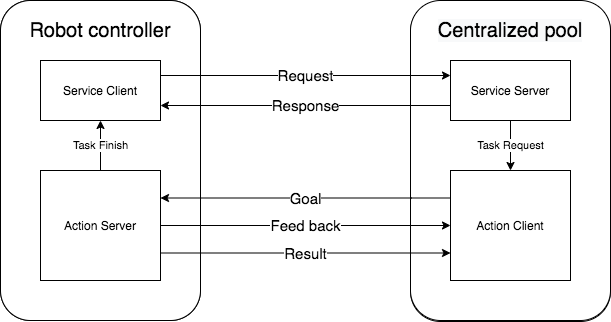
\includegraphics[width = 0.7\textwidth]{content/images/ch4/robot_pool_comminication.drawio.png}
    \caption{Communication between Robot and Centralized Pool}
    \label{fig:comminication}
\end{figure}

\begin{table}[htb]
\centering
\begin{tabular}{|c|c|c|} 
\hline
Battery & Pose & Robot id\\
\hline\hline
93	&(2,4)	&1 \\ [1ex] 
\hline
\end{tabular}
\caption{Request Message Format and Example}
\label{tab:request_message}
\end{table}

\begin{table}[htb]
\centering
\begin{tabular}{|c|c|c|c|} 
\hline
Task id[] &Task type & Target id & Goal[] \\
\hline\hline
1& Gather Environment Info & 9	& (-1.5,5.2) 2020-06-01 9:00:00 \\
\hline
[3,4]	& Execute task & 21, 22	& (-24.0,12.0), 2020-06-01 9:02:00 (-21.0,12.0) 2020-06-01 9:02:00 \\
\hline
5	& Charging	& 17	&(0.0,5.0), 2020-06-01 9:04:00 \\ [1ex] 
\hline
\end{tabular}
\caption{Action Goal Message Format and Example}
\label{tab:goal_message}
\end{table}

\begin{table}[htb]
\centering
\begin{tabular}{|c|c|c|c|} 
\hline
Robot id & Door id & Measurement time & Measurement result \\
\hline\hline
1	& 3	& 2020-06-01 9:00:03 & Door open \\ [1ex] 
\hline
\end{tabular}
\caption{Action Feedback Message Format and Example}
\label{tab:feedback_message}
\end{table}

\begin{table}[htb]
\centering
\begin{tabular}{|c|c|c|} 
\hline
Task id	& Task type	& Result\\
\hline\hline
1 & Gather Enviroment Info & Success \\ [1ex] 
\hline
\end{tabular}
\caption{Action Result Message Format and Example}
\label{tab:result_message}
\end{table}







\section{Database}
F
\begin{figure}[htbp]
    \centering
    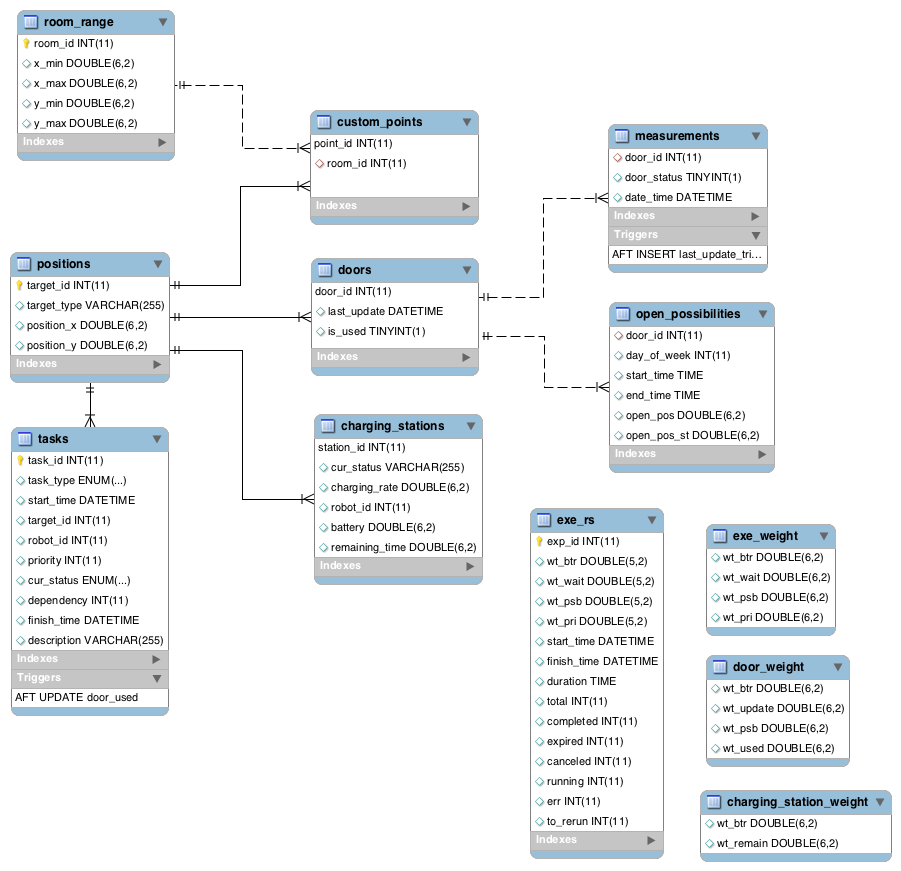
\includegraphics[width = 0.7\textwidth]{content/images/ch4/database_er.png}
    \caption{Database Entity Relationship Diagram}
    \label{}
\end{figure}



\section{Procedure}
Each robot autonomously request task from the centralized pool and centralized pool response with a set of suitable tasks. 
\subsection{Robot}
\paragraph{Robot Component} The robot component is shown in Figure \ref{fig:robot_components}. The following are explanations of some robot components.


\begin{figure}[htbp]
	\centering
	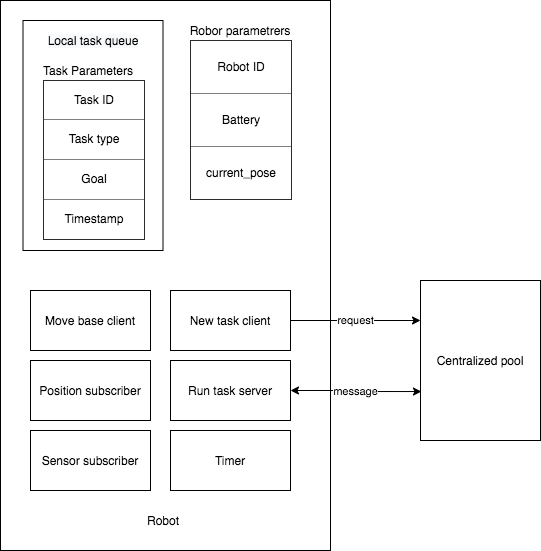
\includegraphics[width = 0.45\textwidth]{content/images/ch4/system_component_robot.drawio.png}
	\caption{Robot Components}
	\label{fig:robot_components}
\end{figure}

\begin{itemize}
	\item \textsl{Battery level.} Battery level drops as the robot moves and rotates.
	\item \textsl{Local task queue.} Local task queue keeps a list of tasks that a robot will run sequentially. Once a task is finished, it would be removed from task queue. Once this queue become empty, the robot send task result to centralized pool.
	\item \textsl{New task client.} Once all task are finished, the new task client send request to new task server.
	\item \textsl{Run task server.} The run task server receive tasks and send task feedback and task result.
	\item \textsl{Timer.} To prevent robot to be hanged by one task forever, the timer check the robot moving state periodically.
	\item \textsl{Move base client.} The move\_base node provides a ROS interface for configuring, running, and interacting with the navigation stack on a robot. The move\_base client send a goal to move\_base node to tracking their status  
	\item \textsl{Position subscriber.} The position subscriber get robot current position from navigation stack. The robot send its current location to centralized pool to request a new task.
	\item \textsl{Sensor subscriber.} The Sensor subscriber listen to sensor data within the range.
\end{itemize}

\paragraph{Robor Task Processing} The flowchart of robot task processing is shown in Figure \ref{fig:robot_task_processing}.

\begin{figure}[htbp]
    \centering
    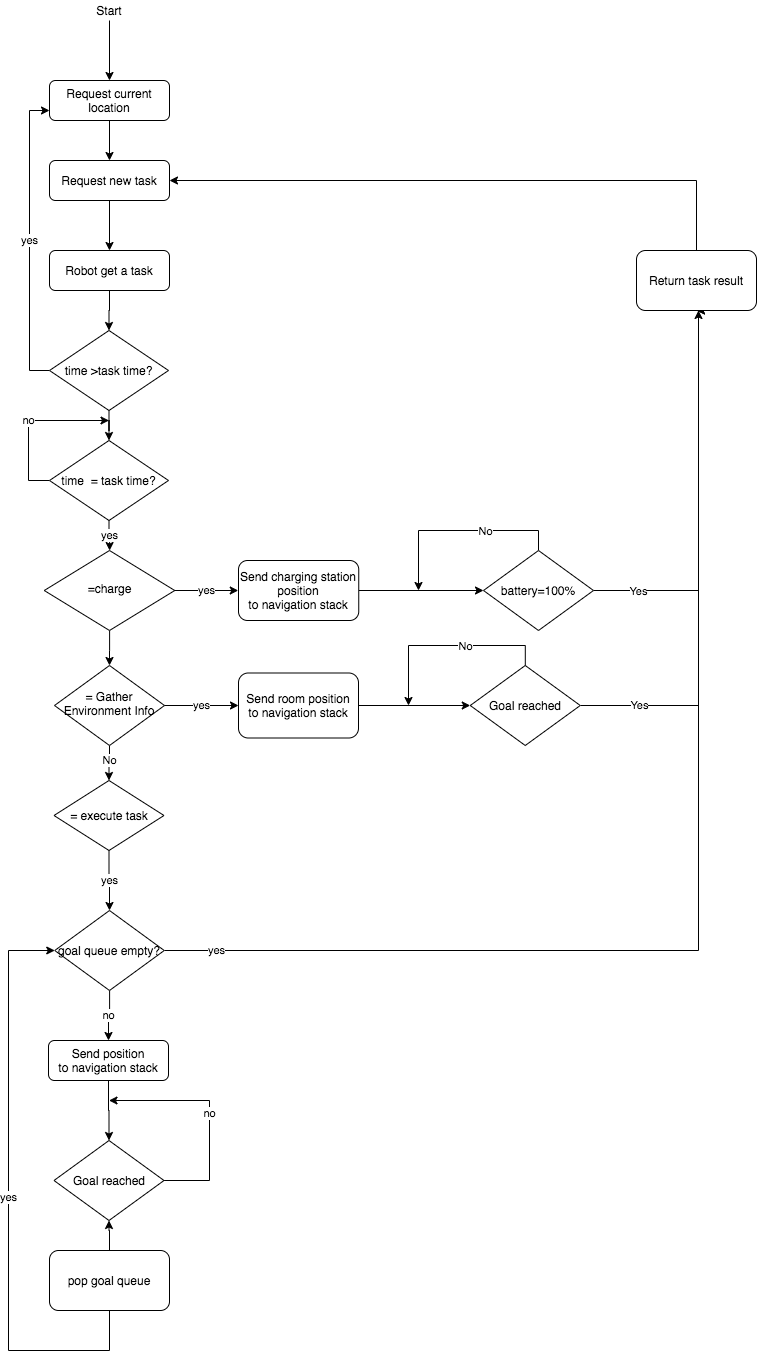
\includegraphics[width = 0.7\textwidth]{content/images/ch4/robot_task_flow.drawio.png}
    \caption{Robot Task Processing Flowchart}
    \label{fig:robot_task_processing}
\end{figure}


\subsection{Centralized Pool}



\begin{itemize}
	\item \textsl{Map Information.} Map information contains information such as the door list that the robot will pass through when moving to target position.
	\item \textsl{Cost calculator.} Cost calculator calculate the cost for doors, rooms and charging stations.
	\item \textsl{Task manager.} Task manager can construct, sort and allocate tasks.
\end{itemize}
\begin{figure}[htbp]
	\centering
	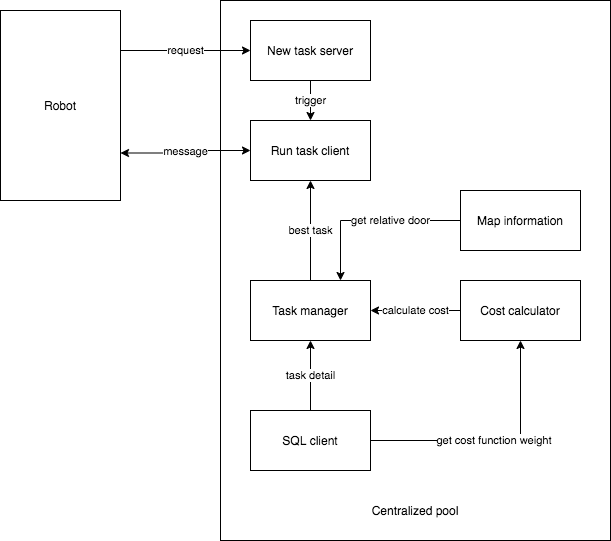
\includegraphics[width = 0.45\textwidth]{content/images/ch4/system_component_centralized_pool.drawio.png}
	\caption{Centralized Pool Components}
	\label{fig:centralized_pool_components}
\end{figure}




\subsection{Charging Station}
\label{sec:charging_station}